\documentclass[12pt,dvipdfmx]{beamer}
\institute{}
\author{田浦健次朗}
\date{}

\usepackage{graphicx}
\DeclareGraphicsExtensions{.pdf}
\DeclareGraphicsExtensions{.eps}
\graphicspath{{out/}{out/tex/}{out/tex/gpl/}{out/tex/svg/}{out/tex/lsvg/}{out/tex/dot/}}
% \graphicspath{{out/}{out/tex/}{out/pdf/}{out/eps/}{out/tex/gpl/}{out/tex/svg/}{out/pdf/dot/}{out/pdf/gpl/}{out/pdf/img/}{out/pdf/odg/}{out/pdf/svg/}{out/eps/dot/}{out/eps/gpl/}{out/eps/img/}{out/eps/odg/}{out/eps/svg/}}
\usepackage{listings,jlisting}
\usepackage{fancybox}
\usepackage{hyperref}
\usepackage{color}

%%%%%%%%%%%%%%%%%%%%%%%%%%%
%%% themes
%%%%%%%%%%%%%%%%%%%%%%%%%%%
\usetheme{default} % Szeged
%% no navigation bar
% default boxes Bergen Boadilla Madrid Pittsburgh Rochester
%% tree-like navigation bar
% Antibes JuanLesPins Montpellier
%% toc sidebar
% Berkeley PaloAlto Goettingen Marburg Hannover Berlin Ilmenau Dresden Darmstadt Frankfurt Singapore Szeged
%% Section and Subsection Tables
% Copenhagen Luebeck Malmoe Warsaw

%%%%%%%%%%%%%%%%%%%%%%%%%%%
%%% innerthemes
%%%%%%%%%%%%%%%%%%%%%%%%%%%
% \useinnertheme{circles}	% default circles rectangles rounded inmargin

%%%%%%%%%%%%%%%%%%%%%%%%%%%
%%% outerthemes
%%%%%%%%%%%%%%%%%%%%%%%%%%%
% outertheme
% \useoutertheme{default}	% default infolines miniframes smoothbars sidebar sprit shadow tree smoothtree


%%%%%%%%%%%%%%%%%%%%%%%%%%%
%%% colorthemes
%%%%%%%%%%%%%%%%%%%%%%%%%%%
\usecolortheme{seahorse}
%% special purpose
% default structure sidebartab 
%% complete 
% albatross beetle crane dove fly seagull 
%% inner
% lily orchid rose
%% outer
% whale seahorse dolphin

%%%%%%%%%%%%%%%%%%%%%%%%%%%
%%% fontthemes
%%%%%%%%%%%%%%%%%%%%%%%%%%%
\usefonttheme{serif}  
% default professionalfonts serif structurebold structureitalicserif structuresmallcapsserif

%%%%%%%%%%%%%%%%%%%%%%%%%%%
%%% generally useful beamer settings
%%%%%%%%%%%%%%%%%%%%%%%%%%%
% 
\AtBeginDvi{\special{pdf:tounicode EUC-UCS2}}
% do not show navigation
\setbeamertemplate{navigation symbols}{}
% show page numbers
\setbeamertemplate{footline}[frame number]

%%%%%%%%%%%%%%%%%%%%%%%%%%%
%%% define some colors for convenience
%%%%%%%%%%%%%%%%%%%%%%%%%%%

\newcommand{\mido}[1]{{\color{green}#1}}
\newcommand{\mura}[1]{{\color{purple}#1}}
\newcommand{\ore}[1]{{\color{orange}#1}}
\newcommand{\ao}[1]{{\color{blue}#1}}
\newcommand{\aka}[1]{{\color{red}#1}}

\setbeamercolor{ex}{bg=cyan!20!white}

\definecolor{UniBlue}{RGB}{20,20,250} 
\setbeamercolor{structure}{fg=UniBlue} % 見出しカラー

\iffalse
%%%%%%%%%%%%%%%%%%%%%%%%%%%
%% customize beamer template
%% https://www.opt.mist.i.u-tokyo.ac.jp/~tasuku/beamer.html
%%%%%%%%%%%%%%%%%%%%%%%%%%%

%\renewcommand{\familydefault}{\sfdefault}  % 英文をサンセリフ体に
%\renewcommand{\kanjifamilydefault}{\gtdefault}  % 日本語をゴシック体に
\usefonttheme{structurebold} % タイトル部を太字
\setbeamerfont{alerted text}{series=\bfseries} % Alertを太字
\setbeamerfont{section in toc}{series=\mdseries} % 目次は太字にしない
\setbeamerfont{frametitle}{size=\Large} % フレームタイトル文字サイズ
\setbeamerfont{title}{size=\LARGE} % タイトル文字サイズ
\setbeamerfont{date}{size=\small}  % 日付文字サイズ

\definecolor{UniBlue}{RGB}{0,150,200} 
\definecolor{AlertOrange}{RGB}{255,76,0}
\definecolor{AlmostBlack}{RGB}{38,38,38}
\setbeamercolor{normal text}{fg=AlmostBlack}  % 本文カラー
\setbeamercolor{structure}{fg=UniBlue} % 見出しカラー
\setbeamercolor{block title}{fg=UniBlue!50!black} % ブロック部分タイトルカラー
\setbeamercolor{alerted text}{fg=AlertOrange} % \alert 文字カラー
\mode<beamer>{
    \definecolor{BackGroundGray}{RGB}{254,254,254}
    \setbeamercolor{background canvas}{bg=BackGroundGray} % スライドモードのみ背景をわずかにグレーにする
}


%フラットデザイン化
\setbeamertemplate{blocks}[rounded] % Blockの影を消す
\useinnertheme{circles} % 箇条書きをシンプルに
\setbeamertemplate{navigation symbols}{} % ナビゲーションシンボルを消す
\setbeamertemplate{footline}[frame number] % フッターはスライド番号のみ

%タイトルページ
\setbeamertemplate{title page}{%
    \vspace{2.5em}
    {\usebeamerfont{title} \usebeamercolor[fg]{title} \inserttitle \par}
    {\usebeamerfont{subtitle}\usebeamercolor[fg]{subtitle}\insertsubtitle \par}
    \vspace{1.5em}
    \begin{flushright}
        \usebeamerfont{author}\insertauthor\par
        \usebeamerfont{institute}\insertinstitute \par
        \vspace{3em}
        \usebeamerfont{date}\insertdate\par
        \usebeamercolor[fg]{titlegraphic}\inserttitlegraphic
    \end{flushright}
}
\fi

%%%%%%%%%%%%%%%%%%%%%%%%%%%
%%% how to typset code
%%%%%%%%%%%%%%%%%%%%%%%%%%%

\lstset{language = C,
numbers = left,
numberstyle = {\tiny \emph},
numbersep = 10pt,
breaklines = true,
breakindent = 40pt,
frame = tlRB,
frameround = ffft,
framesep = 3pt,
rulesep = 1pt,
rulecolor = {\color{blue}},
rulesepcolor = {\color{blue}},
flexiblecolumns = true,
keepspaces = true,
basicstyle = \ttfamily\scriptsize,
identifierstyle = ,
commentstyle = ,
stringstyle = ,
showstringspaces = false,
tabsize = 4,
escapechar=\@,
}

\AtBeginSection[]
{
\begin{frame}
\frametitle{}
\tableofcontents[currentsection]
\end{frame}
}

\AtBeginSubsection[]
{
\begin{frame}
\frametitle{}
\tableofcontents[currentsection,currentsubsection]
\end{frame}
}


\title{並行処理と同期}

\AtBeginSection[]
{
\begin{frame}
\frametitle{Contents}
\tableofcontents[currentsection]
\end{frame}
}

\AtBeginSubsection[]
{
\begin{frame}
\frametitle{Contents}
\tableofcontents[currentsection,currentsubsection]
\end{frame}
}

\begin{document}
\maketitle

%%%%%%%%%%%%%%%%%%%%%%%%%%%%%%%%%% 
\begin{frame}
\frametitle{目次}
\tableofcontents
\end{frame}

%%%%%%%%%%%%%%%%% 
\section{共有メモリと競合状態}
%%%%%%%%%%%%%%%%% 

%%%%%%%%%%%%%%%%% 
\begin{frame}[fragile]
  \frametitle{共有メモリ}
  \begin{itemize}
  \item (復習) 同一プロセス内のスレッドはメモリを共有している
  \item 例えば以下のプログラムは何を表示する?

\begin{lstlisting}
/* 大域変数 */
int @\mura{\tt g}@ = 0;

/* スレッドの開始関数 */
void * f(void * arg) {
  @\mura{\tt g += 100;}@
  return 0; }

int main() {
  @\mura{\tt g = 200;}@
  /* スレッドを作る */
  pthread_t child_thread_id;
  pthread_create(&child_thread_id, 0, f, 0);
  /* 終了待ち */
  void * ret = 0;
  pthread_join(child_thread_id, &ret);
  printf("g = %d\n", @\mura{\tt g}@); /* ここで表示されるのは? */
  return 0;
}
\end{lstlisting} 
  \end{itemize}
\end{frame} 

%%%%%%%%%%%%%%%%% 
\begin{frame}[fragile]
  \frametitle{次のプログラムは?}
  \begin{itemize}
  \item 違い: 2つの子スレッドを作る ({\tt f}は先と同じ)
\begin{lstlisting}
int main() {
  int err;
  @\mura{\tt g = 200;}@
  /* スレッドを作る */
  pthread_t child_thread_id[2];
  for (int i = 0; i < 2; i++)
    pthread_create(&child_thread_id[i], 0, f, 0);
  /* 終了待ち */
  for (int i = 0; i < 2; i++) {
    void * ret = 0;
    pthread_join(child_thread_id[i], &ret);
  }
  printf("g = %d\n", @\mura{\tt g}@);
  return 0;
}
\end{lstlisting} 
\end{itemize}
\end{frame}

%%%%%%%%%%%%%%%%% 
\begin{frame}
  \frametitle{望む結果(400)にならない実行系列}
  \begin{center}
\begin{tabular}{l|l|l}
    & 子スレッドA                   &  子スレッドB                   \\
A1: & $t_0$ {\tt = g} (200){\tt ;}  &                                \\
B1: &                               &  $t_1$ {\tt = g} (200){\tt ;}  \\
B2: &                               &  {\tt g = 300;}                \\
A2: &  {\tt g = 300;}               &                                \\
\end{tabular}
  \end{center}

\begin{itemize}
\item 他にも様々なケースが考えられる(e.g., A1; B1; A2; B2)
\item うまく行くのは以下の2ケースのみ
  \begin{itemize}
  \item A1; A2; B1; B2;
  \item B1; B2; A1; A2;
  \end{itemize}

\item 言葉で言えば, うまく行く
  $\iff$ 片方の\ao{{\tt g += 100}の間にもう一方のスレッドによって
  {\tt g}が書き換えられていない}
\end{itemize}
\end{frame}

%%%%%%%%%%%%%%%%% 
\begin{frame}
  \frametitle{注: 問題の根本}
  \begin{itemize}
  \item {\tt g += 100}が「実は」

    \begin{tabular}{l}
      $t$ {\tt = g;} \\
      {\tt g = $t$ + 100;} \\
    \end{tabular}

    の二つの文に分かれて実行されていると聞いて,
    「他にもやり方はあるかも知れない, なぜそのように決めつけるのだ?」
    と思うのは正しい疑問
    
  \item より本質的な問題の記述は以下
    \begin{itemize}
    \item CPUが「一度に」行えるメモリに対する操作は,  read (load命令),
      write (store命令)\ao{そのどちらか}である
    \item そのもとで,
      ある変数に対する加算を複数のスレッドが「確実に」行うには?
    \end{itemize}
  \end{itemize}
\end{frame}

%%%%%%%%%%%%%%%%% 
\begin{frame}[fragile]
  \frametitle{より単純な例でも問題がある}
  \begin{itemize}
  \item スレッド$W$からスレッド$R$へ値を伝える
  \item $W$が変数{\tt x}に値を書き込んで$R$がそれを読む
    \begin{columns}
      \begin{column}{0.1\textwidth}
      \end{column}
      \begin{column}{0.4\textwidth}
スレッド$W$        
\begin{lstlisting}
{
  ...
  x = @{\it answer}@;
}
\end{lstlisting}
      \end{column}
      \begin{column}{0.1\textwidth}
      \end{column}
      \begin{column}{0.4\textwidth}
スレッド$R$
\begin{lstlisting}
{  
  @{\it a}@ = x;
  ...
}
\end{lstlisting}
      \end{column}
    \end{columns}

    \begin{columns}
      \begin{column}{0.5\textwidth}
lucky:
        
\begin{tabular}{l|l}
スレッド$W$          & スレッド$R$    \\
{\tt x = }$a${\tt ;} &                \\
                     & $t$ {\tt = x;} \\
\end{tabular}
      \end{column}
      \begin{column}{0.5\textwidth}
unlucky:
        
\begin{tabular}{l|l}
スレッド$W$          & スレッド$R$    \\
                     & $t$ {\tt = x;} \\
{\tt x = }$a${\tt ;} &                \\
\end{tabular}
      \end{column}
    \end{columns}
\end{itemize}
\end{frame}

\iffalse
%%%%%%%%%%%%%%%%% 
\begin{frame}
  \frametitle{用語: 生産者消費者同期 (producer-consumer synchronization)}
  \begin{itemize}
  \item 値を計算($=$生産)するスレッドから使用($=$消費)するスレッドへ,
    正しくデータを受け渡す
  \end{itemize}

  
  これらを見ると, メモリを共有しているから簡単に
  通信(データ共有)が出来るというわけではなさそうとわかる

\end{frame}
\fi


%%%%%%%%%%%%%%%%% 
\begin{frame}
  \frametitle{用語: 競合状態}
  \begin{itemize}
  \item [] 定義: 以下のような状態を「競合状態」という
    \begin{enumerate}
    \item 複数のスレッドが
      \underline{(a) 同じ場所(変数, 配列, 構造体の要素 etc.)}を, 
      \underline{(b) 並行して}
      アクセスしている
    \item うち少なくとも1つは書き込みである
    \end{enumerate}
  \item 競合状態があるプログラムは, 
    \begin{itemize}
    \item ほとんどの場合, 非決定的: 実行のタイミングによって結果が異なり,
      うち一部しか「望ましい」結果ではない
    \item $\Rightarrow$ うまく動かないことがあり得る
    \end{itemize}
  \item 用語: \ao{際どい領域 (critical section)}
    コード上で, 競合状態が発生している領域
  \end{itemize}
\end{frame}

%%%%%%%%%%%%%%%%% 
\begin{frame}
  \frametitle{競合状態を大雑把に分類}
  \begin{itemize}
  \item \mura{不可分性(atomicity)}の崩れ:
    \begin{itemize}
    \item \ao{「一度にできない一連の操作」}の途中に,
      他の処理(更新)が挟まるために, 意図した操作が行えなくなる状態
    \item \ao{「一度にできない一連の操作」}の例
      \begin{itemize}
      \item 1つの変数を\mura{読み出し〜変更}
      \item \mura{2つ以上の変数}を読み出し, または書き込み
      \end{itemize}
    \item 用語「一度に出来る」$\approx$ 他の処理が挟まらないことが
      保証されている $\equiv$ \ao{不可分(atomic)}に実行できる
    \end{itemize}
    
  \item \mura{順序, 依存関係 (dependency)}の崩れ:
    \begin{itemize}
    \item 複数スレッド間で, 読み書きにある順序
      (例えば書いてから読む)を保証しなくてはならないが,
      それが崩れるために意図した値の通信が行えなくなる状態
    \end{itemize}    
  \end{itemize}
\end{frame}

%%%%%%%%%%%%%%%%% 
\section{同期}
%%%%%%%%%%%%%%%%% 
\begin{frame}
  \frametitle{同期 (synchronization)}
  \begin{itemize}
  \item 一般的な意味: 歩調を合わせる, タイミングをそろえる
  \item 並行処理という文脈での意味:
    \ao{競合状態を避けるための, タイミングの制御}
  \end{itemize}
\end{frame}

%%%%%%%%%%%%%%%%% 
\begin{frame}
  \frametitle{同期の種類}
  \begin{itemize}
  \item \ao{排他制御} (目的: 不可分性の保証)
  \item \ao{バリア同期} (多スレッド間で順序を保証)
  \item \ao{条件変数} (目的:
    順序の保証含め, 「何かが起きるまで待ってから実行」
    をするための\ao{汎用機構})
  \end{itemize}
\end{frame}

\subsection{排他制御}

%%%%%%%%%%%%%%%%% 
\begin{frame}[fragile]
  \frametitle{排他制御 (mutual exclusion; \ao{mutex})}
  \begin{itemize}
  \item 排他制御 $\approx$ 一人しか入れない部屋(個室トイレ)
  \item 排他制御に対する操作
    \begin{itemize}
    \item \ao{lock} $\approx$ トイレが空いていれば入って鍵をかける;
      空いていなければ空くまでで待つ
    \item \ao{unlock} $\approx$ 鍵を開けてトイレを空ける
    \end{itemize}
  \item 典型的な使い方(不可分に行いたい操作をlock/unlockではさむ)
    \begin{columns}
      \begin{column}{0.5\textwidth}
\begin{lstlisting}
lock(...);
  操作
unlock(...);
\end{lstlisting}
      \end{column}
      \begin{column}{0.5\textwidth}
        \begin{center}

\includegraphics[width=0.7\textwidth]{out/pdf/img/kasetsu_toilet.pdf}
        \end{center}
      \end{column}
    \end{columns}
  \end{itemize}
\end{frame}

%%%%%%%%%%%%%%%%% 
\begin{frame}
  \frametitle{Pthreadのmutex API}
  \begin{itemize}
  \item {\tt \#include <pthread.h>}
  \item {\tt pthread\_mutex\_t m;} /* 排他制御オブジェクト */
  \item {\tt pthread\_mutex\_init(\&m, attr);}
  \item {\tt pthread\_mutex\_destroy(\&m);}
  \item \ao{\tt pthread\_mutex\_lock(\&m);}   /* lock */
  \item {\tt pthread\_mutex\_try\_lock(\&m);}
  \item \ao{\tt pthread\_mutex\_unlock(\&m);} /* unlock */
  \end{itemize}
\end{frame}

%%%%%%%%%%%%%%%%% 
\begin{frame}[fragile]
  \frametitle{Mutex APIによって保証されること}
  \begin{itemize}
  \item あるmutex $m$に対して,
    {\tt pthread\_mutex\_lock({\it m})}
    と{\tt pthread\_mutex\_unlock({\it m})}
    に挟まれた(前者がreturnしてから後者を呼び出すまでの)時間帯
    を「$m$による排他区間」と呼ぶことにする
    \begin{columns}
      \begin{column}{0.5\textwidth}
\begin{lstlisting}
pthread_mutex_lock(@$m$@);
  ...
pthread_mutex_unlock(@$m$@);
\end{lstlisting}
      \end{column}
      \begin{column}{0.5\textwidth}
        \begin{center}
\only<1>{\includegraphics[width=0.8\textwidth]{out/pdf/svg/mutex_1.pdf}}%
\only<2>{\includegraphics[width=0.8\textwidth]{out/pdf/svg/mutex_2.pdf}}%
\only<3>{\includegraphics[width=0.8\textwidth]{out/pdf/svg/mutex_3.pdf}}
        \end{center}
      \end{column}
    \end{columns}
\item 保証: 同一の$m$に対する排他区間は時間的に重ならない
  \end{itemize}
\end{frame}

%%%%%%%%%%%%%%%%% 
\begin{frame}[fragile]
  \frametitle{最初の間違いの修正}
  \begin{itemize}
  \item []
\begin{lstlisting}
void * f(void * arg) {
  @\mura{\tt g += 100;}@
  return 0; }
\end{lstlisting}
\item [] $\Rightarrow$
\begin{lstlisting}
@\mura{\tt pthread\_mutex\_t m;}@
    
void * f(void * arg) {
  @\mura{\tt pthread\_mutex\_lock(\&m);}@
  g += 100;
  @\mura{\tt pthread\_mutex\_unlock(\&m);}@
  return 0;
}

int main() {
  @\mura{\tt pthread\_mutex\_init(\&m, attr);}@
  ...
}
\end{lstlisting}
\end{itemize}
\end{frame}

%%%%%%%%%%%%%%%%% 
\begin{frame}[fragile]
  \frametitle{同期を隠蔽したデータ構造}
  \begin{itemize}
  \item データをスレッドで更新する必要性が生ずるたびに,
    mutexを別途定義するのは煩わしい・間違いの元
  \item データ $+$ それを保護するmutex (または今後述べる同期のためのデータ)
    をひとつのデータ構造に隠蔽するのが通常
    (\ao{スレッドセーフ}なデータ構造・関数)
  \item 例
\begin{lstlisting}
typedef struct {
  int x;             // 更新される変数
  pthread_mutex_t m; // xを守るためのmutex
} counter_t;
int counter_inc(counter_t * c, int dx) {
  pthread_mutex_lock(&c->m);
  int x = c->x;
  c->x = x + dx;
  pthread_mutex_unlock(&c->m);
  return x;
}
\end{lstlisting}
\end{itemize}
\end{frame}

\subsection{バリア同期}
%%%%%%%%%%%%%%%%% 
\begin{frame}
  \frametitle{バリア同期}
  \begin{itemize}
  \item バリア $\approx$ 出走馬のゲート(発馬機)
  \item 全員が揃うまで待ち, そろったら一斉に開ける
    \begin{center}
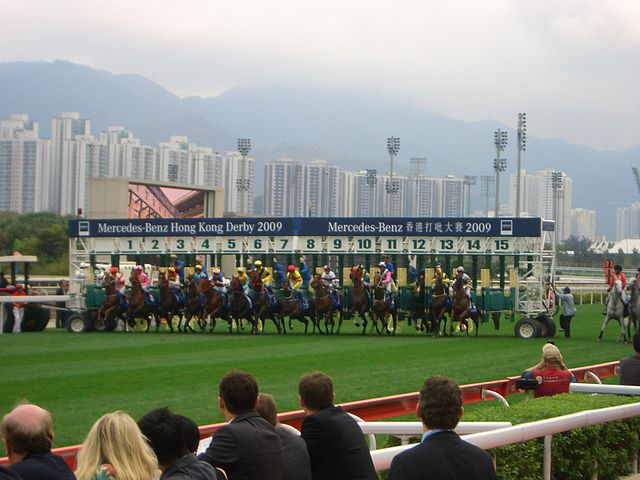
\includegraphics[width=0.4\textwidth]{out/pdf/img/Hong_Kong_Derby.pdf}

{\tiny\url{https://commons.wikimedia.org/w/index.php?curid=6317140}}
\end{center}
\end{itemize}
\end{frame}

%%%%%%%%%%%%%%%%% 
\begin{frame}
  \frametitle{PthreadのバリアAPI}
  \begin{itemize}
  \item {\tt \#include <pthread.h>}
  \item {\tt pthread\_barrier\_t b;}  /* バリアオブジェクト */
  \item {\tt pthread\_barrier\_init(\&b, attr, count);}

    /* {\tt count=}参加するスレッド数 */
  \item {\tt pthread\_barrier\_destroy(\&b);}
  \item \ao{\tt pthread\_barrier\_wait(\&b);}

    /* 同期点に到達; 他のスレッドを待つ */
  \end{itemize}
\end{frame}

%%%%%%%%%%%%%%%%% 
\begin{frame}[fragile]
  \frametitle{バリアAPIによって保証されること}
  \begin{itemize}
  \item [] $b$ : {\tt count = }$n$で初期化されたバリアオブジェクト
  \item $n$スレッドが{\tt pthread\_barrier\_wait($b$)}
    を呼び出すまで, どの呼び出しもリターンしない
  \item 実践的な意味: {\tt pthread\_barrier\_wait($b$)}を
    \begin{itemize}
    \item 呼び出す前($A$)の書き込み$\rightarrow$リターン後($B$)の読み込みに伝わる
    \item 呼び出す前($A$)の読み込み$\rightarrow$
      リターンした後($B$)の値は読まない(前の値が潰されている心配はない)
    \end{itemize}
  \end{itemize}

  \begin{columns}
    \begin{column}{0.4\textwidth}
      \begin{lstlisting}
  ... (@$A$@) ...
barrier_wait(b);        
  ... (@$B$@) ...
      \end{lstlisting}
    \end{column}
    \begin{column}{0.5\textwidth}
      \begin{center}
        \only<1>{\includegraphics[width=\textwidth]{out/pdf/svg/barrier_1.pdf}}%
        \only<2>{\includegraphics[width=\textwidth]{out/pdf/svg/barrier_2.pdf}}%
        \only<3>{\includegraphics[width=\textwidth]{out/pdf/svg/barrier_3.pdf}}%
      \end{center}
    \end{column}
  \end{columns}
\end{frame}

%%%%%%%%%%%%%%%%% 
\subsection{条件変数}
\begin{frame}
  \frametitle{条件変数(condition variable)}
  \begin{itemize}
  \item 条件変数$\approx$布団
  \item 「ある条件が整うまで待つ」, 「待っているスレッドを起こす」
    ための汎用同期機構

    \begin{center}

\includegraphics[width=0.4\textwidth]{out/pdf/img/futon.pdf}
\end{center}
    
  \end{itemize}
\end{frame}

%%%%%%%%%%%%%%%%% 
\begin{frame}
  \frametitle{Pthreadの条件変数API}
  \begin{itemize}
  \item {\tt \#include <pthread.h>}
  \item {\tt pthread\_cond\_t c;}
  \item {\tt pthread\_cond\_init(\&c, attr);}
  \item {\tt pthread\_cond\_destroy(\&c);}
  \item \ao{\tt pthread\_cond\_wait(\&c, \&m);} /* 寝る */
    \begin{itemize}
    \item {\tt pthread\_mutex\_t m;}
    \end{itemize}
  \item \ao{\tt pthread\_cond\_broadcast(\&c);} /* 全員起こす */
  \item \ao{\tt pthread\_cond\_signal(\&c);}    /* 誰か一人起こす */
  \end{itemize}
\end{frame}

%%%%%%%%%%%%%%%%% 
\begin{frame}
  \frametitle{{\tt pthread\_cond\_wait($c$, $m$)}の動作}
  \begin{itemize}
  \item {\tt pthread\_cond\_wait($c$, $m$)}を呼び出したスレッドが$m$をロックしていることが前提. その上で, 
    \begin{itemize}
    \item<2-> $m$をunlockする
    \item<2-> $c$の上で寝る(中断・ブロックする)
    \end{itemize}
  \item [] <2->{を\mura{不可分に}行う}
    \begin{itemize}
    \item<3-> 目覚めてリターンする際はまた$m$をlockしている
    \end{itemize}
\begin{center}
\only<1>{\includegraphics[width=0.9\textwidth]{out/pdf/svg/cond_wait_1.pdf}}%
\only<2>{\includegraphics[width=0.9\textwidth]{out/pdf/svg/cond_wait_2.pdf}}%
\only<3->{\includegraphics[width=0.9\textwidth]{out/pdf/svg/cond_wait_3.pdf}}%
\end{center}
  \item<4-> この一見複雑な動作の意味は後にわかる
  \end{itemize}
\end{frame}

%%%%%%%%%%%%%%%%% 
\begin{frame}[fragile]
  \frametitle{例: 飽和するカウンタ}
  \begin{itemize}
  \item 例として以下のようなAPIを実現することを考える
\begin{lstlisting}
typedef struct { ... } scounter_t;

/* 初期化. 飽和する値capacityを指定. カウンタの初期値を0にセット */
int scounter_init(scounter_t * s, int capacity);

/* +1; @\mura{ただしcapacityを超える場合は(誰かがdecしてくれるのを)待つ}@ */
int scounter_inc(scounter_t * s);

/* -1; 簡単のため0を下回ってもよい */
int scounter_dec(scounter_t * s);
\end{lstlisting}
\item inc, decとも複数のスレッドが並行に呼び出し得る
  (それでも正しく動作する. i.e., スレッドセーフ)
\end{itemize}
\end{frame}

%%%%%%%%%%%%%%%%% 
\begin{frame}[fragile]
  \frametitle{飽和なし版}
  \begin{itemize}
  \item データ構造 (mutexを隠蔽)
\begin{lstlisting}
typedef struct {
  @\mura{\tt pthread\_mutex\_t m;}@
  int x;
  int capacity;
} scounter_t;
\end{lstlisting}
  \item inc (足し算を不可分に)
\begin{lstlisting}
int scounter_inc(scounter_t * s) {
  pthread_mutex_lock(&s->m);
  int x = s->x;
  s->x = x + 1;
  pthread_mutex_unlock(&s->m);
  return x;
}
\end{lstlisting}
\end{itemize}
\end{frame}

%%%%%%%%%%%%%%%%% 
\begin{frame}[fragile]
  \frametitle{飽和あり版 概要}
  \begin{itemize}
  \item 飽和していたら待機
\begin{lstlisting}
int scounter_inc(scounter_t * s) {
  pthread_mutex_lock(&s->m);
  int x = s->x;
  @\ao{\tt if (x == s->capacity) \{}@
    @\ao{\tt ... 待機 ...}@
  @\ao{\}}@
  pthread_mutex_unlock(&s->m);
  return x;  }
\end{lstlisting}
\item 上記の「待機」をするのが {\tt pthread\_cond\_wait}
\item しかし上記では起こされた以降の動作が不足している
\item $\rightarrow$ \ao{目覚めたらまたやり直す}コード(ループ)に変形
  \end{itemize}
\end{frame}

%%%%%%%%%%%%%%%%% 
\begin{frame}[fragile]
  \frametitle{飽和あり版 概要}
  \begin{itemize}
  \item []
\begin{lstlisting}
int scounter_inc(scounter_t * s) {
  pthread_mutex_lock(&s->m);
  int x;
  @\ao{\tt while (1) \{}@
    x = s->x;
    if (x < s->capacity) break;
    @\ao{\tt pthread\_cond\_wait(\&s->c, \&s->m); /* 待機 */}@
  @\ao{\tt \}}@
  /* 仕事が可能になった */
  s->x = x + 1;
  pthread_mutex_unlock(&s->m);
  return x;
}
\end{lstlisting}
\end{itemize}
\end{frame}

%%%%%%%%%%%%%%%%% 
\begin{frame}[fragile]
  \frametitle{飽和あり版 dec}
  \begin{itemize}
  \item $-1$したことで飽和状態が解消されたら,
    寝ている人を(いれば)起こす
    \begin{lstlisting}
int scounter_dec(scounter_t * s) {
  pthread_mutex_lock(&s->m);
  int x = s->x;
  s->x = x - 1;
  if (x == s->capacity) {
    @\mura{\tt pthread\_cond\_broadcast(\&s->c);}@
  }
  pthread_mutex_unlock(&s->m);
  return x;
}
    \end{lstlisting}
  \end{itemize}
\end{frame}

%%%%%%%%%%%%%%%%% 
\begin{frame}[fragile]
  \frametitle{{\tt pthread\_cond} \mura{\tt \_signal} vs \mura{\tt \_broadcast}}
  \begin{itemize}
  \item broadcast($c$) : $c$上で寝ている人を全員起こす
  \item signal($c$) : $c$上で寝ている人のうちどれか一人を起こす
  \item 「誰が起きてもいい」と確信出来る場合はsignal, そうでなければ
    broadcastを使う
  \end{itemize}

\end{frame}

%%%%%%%%%%%%%%%%% 
\begin{frame}[fragile]
  \frametitle{条件変数の使い方テンプレート}
  \begin{itemize}
  \item 「条件$C$が成り立つまで待って$A$をする」
\begin{lstlisting}
pthread_mutex_lock(&m);
while (1) {
  @$C$@ = ...; /* 条件評価 */
  if (@$C$@) break;
  pthread_cond_wait(&c, &m);
}
/* @$C$@ が成り立っているのでここで何かをする */
@$A$@
/* 寝ている誰かを起こせそうなら起こす */
 ...
pthread_mutex_unlock(&m);      
\end{lstlisting}
\end{itemize}
\end{frame}

%%%%%%%%%%%%%%%%% 
\begin{frame}[fragile]
  \frametitle{{\tt pthread\_cond\_wait($c$, $m$)}の動作}
  \begin{itemize}
  \item {\tt pthread\_cond\_wait}が条件変数だけでなく,
    (lockされたことが前提の) mutex を引数に取るという仕様は一見わかりにくい
    (必然性がわからない)
  \item しかしよく考えると実によく出来ている
\begin{lstlisting}
pthread_mutex_lock(&m);
while (1) {
  @$C$@ = ...; /* 条件評価 */
  if (@$C$@) break;
  pthread_cond_wait(&c, &m);
}
  ...
pthread_mutex_unlock(&m);      
\end{lstlisting}
\end{itemize}
\end{frame}

%%%%%%%%%%%%%%%%% 
\begin{frame}[fragile]
  \frametitle{{\tt pthread\_cond\_wait($c$, $m$)}の動作}
  \begin{itemize}
  \item []
\begin{lstlisting}
pthread_mutex_lock(&m);
while (1) {
  @$C$@ = ...; /* 条件評価 */
  if (@$C$@) break;
  pthread_cond_wait(&c, &m);
}
  ...
pthread_mutex_unlock(&m);      
\end{lstlisting}
\begin{enumerate}
\item<1-> 通常データ構造は, どのみち何らかのmutexで保護されているので,
  条件$C$を判定する際にmutexをlockしているのは自然
\item<2-> しかも自分がブロックする際はそのmutexを開放しないと,
  他のスレッドがデータを変更できない
  ({\tt pthread\_cond\_wait}がそれをやってくれているのは親切)
\item<3-> しかしそれでも, 「unlock」と「寝る」は別のAPIでも良いのではという
  疑問が残る
\end{enumerate}
\end{itemize}
\end{frame}

%%%%%%%%%%%%%%%%% 
\begin{frame}[fragile]
  \frametitle{これでは何がいけないか?}
  \begin{itemize}
  \item {\tt pthread\_cond\_wait*($c$)} : $c$上で寝るだけの(架空の)API
\begin{lstlisting}
pthread_mutex_lock(&m);
while (1) {
  @$C$@ = ...; /* 条件評価 */
  if (@$C$@) break;
  pthread_mutex_unlock(&m); // unlockして
  pthread_cond_wait*(&c);   // 寝る
  pthread_mutex_lock(&m);   // 目覚めたらまたlock
}
  ...
pthread_mutex_unlock(&m);      
\end{lstlisting}
\end{itemize}
\end{frame}

%%%%%%%%%%%%%%%%% 
\begin{frame}[fragile]
  \frametitle{Lost wake up問題}

  \begin{itemize}
  \item<1-> 本来起こされるべき(ブロックしてはならない)人がブロックしてしまう問題
  \item<7-> unlockとブロックが「不可分に」行われれば起きないことに注意
  \end{itemize}

\begin{center}
\only<2>{\includegraphics[width=0.7\textwidth]{out/pdf/svg/lost_wakeup_1.pdf}}%
\only<3>{\includegraphics[width=0.7\textwidth]{out/pdf/svg/lost_wakeup_2.pdf}}%
\only<4>{\includegraphics[width=0.7\textwidth]{out/pdf/svg/lost_wakeup_3.pdf}}%
\only<5>{\includegraphics[width=0.7\textwidth]{out/pdf/svg/lost_wakeup_4.pdf}}%
\only<6->{\includegraphics[width=0.7\textwidth]{out/pdf/svg/lost_wakeup_5.pdf}}%
\end{center}
  
\end{frame}

%%%%%%%%%%%%%%%%% 
\begin{frame}[fragile]
  \frametitle{Lost wake up問題}

  {\footnotesize 注: 関数名は適宜短縮している({\tt pthread\_mutex\_lock} $\rightarrow$ {\tt lock}など)}
  \vskip-5mm
\begin{columns}[t]
  \begin{column}{0.53\textwidth}
    \begin{lstlisting}
inc(s) {
  lock(&s->m);
  while (1) {
    if (s->x < s->capacity) break;
    unlock(&s->m);
    cond_wait*(&s->c, &s->m);
    lock(&s->m); }
  ...
\end{lstlisting}
\end{column}    
\begin{column}{0.5\textwidth}
  \begin{itemize}
  \item []
\begin{lstlisting}
dec(s) {
  lock(&s->m);
  int x = s->x;  s->x = x - 1;
  if (x == s->capacity) {
    cond_broadcast(&s->c);
  }
  unlock(&s->m);
\end{lstlisting}
\end{itemize}
\end{column}
\end{columns}

{\scriptsize
\begin{center}
  {\tt s->x == capacity}
  
\begin{tabular}{|ll|ll|}
   &  inc                            &    & dec                            \\\hline
5: & {\tt if (s->x < s->capacity) ...;} &    &                                \\
6: & {\tt unlock(\&s->m)}            &    &                                \\ 
   &                                 & 2: & {\tt lock(\&s->m)}             \\ 
   &                                 & 3: & {\tt int x = s->x; s->x = x - 1;}  \\
   &                                 & 4: & {\tt if (x == s->capacity) \{} \\
   &                                 & 5: & \ \ \mura{\tt cond\_broadcast(\&s->c)}     \\ 
7: & \mura{\tt wait*(\&s->m)}        &    &                                \\
\end{tabular}
\end{center}}

\begin{itemize}
\item cond\_wait の仕様($m$の開放$+$休眠を「不可分に」行う)は,
  まさにこうならないことを保証している
\end{itemize}

\end{frame}

%%%%%%%%%%%%%%%%% 
\section{不可分更新命令}
%%%%%%%%%%%%%%%%%

%%%%%%%%%%%%%%%%% 
\begin{frame}[fragile]
  \frametitle{不可分更新命令}
  \begin{itemize}
  \item CPUが不可分に行えるのは, 64 bitまでのload, storeのどちらか\mura{($\ast$)}
  \item それ以上の処理の不可分性を保証するための基本は排他制御
\begin{lstlisting}
lock(m);
  ...      
unlock(m);
\end{lstlisting}
\ao{\bf 実は\ldots}
\item  一変数に対する読み書きを不可分に行ういくつかの命令がある
  (つまり\mura{($\ast$)}は正確ではない)
  \begin{itemize}
    \item ad-hocな命令
      \begin{itemize}
      \item fetch\&add
      \item test\&set
      \item swap
      \end{itemize}
    \item 汎用命令
      \begin{itemize}
      \item \ao{compare\&swap}
      \end{itemize}
  \end{itemize}
  \end{itemize}
\end{frame}

%%%%%%%%%%%%%%%%% 
\begin{frame}[fragile]
  \frametitle{ad-hocな不可分更新命令}
  \begin{itemize}
  \item [] それぞれ以下を\ao{不可分に}行う命令
    \begin{itemize}
    \item test\&set $p$ (0だったら1にする)
\begin{lstlisting}
if (@\ao{\tt *$p$}@ == 0) {
  @\ao{\tt *$p$}@ = 1; return 1;
} else {
  return 0;
}
\end{lstlisting}

\item fetch\&add $p$,$x$ 
\begin{lstlisting}
@\ao{\tt *$p$}@ = @\ao{\tt *$p$}@ + x;
\end{lstlisting}

\item swap $p$,$r$
\begin{lstlisting}
x = @\ao{\tt *$p$}@;
@\ao{\tt *$p$}@ = @$r$@;
@$r$@ = x;
\end{lstlisting}
    \end{itemize}
  \end{itemize}

{\scriptsize GCC: \url{https://gcc.gnu.org/onlinedocs/gcc/_005f_005fsync-Builtins.html}}
\end{frame}

%%%%%%%%%%%%%%%%% 
\begin{frame}[fragile]
  \frametitle{compare\&swap (CAS)}
  \begin{itemize}
  \item compare\&swap $p$,$r$,$s$
\begin{lstlisting}
x = @\ao{\tt *$p$}@;
if (x == @$r$@) {
  @\ao{\tt *$p$}@ = @$s$@;
  @$s$@ = x;
}
\end{lstlisting}

\item 自分が読んだ値が書き換わっていないことを確かめながら, 書き込むのに使える
  
\item GCCの関数2種類
  \begin{itemize}
  \item bool {\tt \_\_sync\_bool\_compare\_and\_swap(type *$p$, type $r$, type $s$)}
    (swapが起きたかどうかを返す)
  \item type {\tt \_\_sync\_val\_compare\_and\_swap(type *$p$, type $r$, type $s$)}
    (*$p$に入っていた値を返す)
  \end{itemize}
\end{itemize}
\end{frame}

%%%%%%%%%%%%%%%%% 
\begin{frame}[fragile]
  \frametitle{compare\&swap (CAS)}
  \begin{itemize}
  \item [] ad-hocなプリミティブを包含
    \begin{itemize}
    \item test\&set($p$) $\equiv$
\begin{lstlisting}
return __sync_bool_compare_and_swap(@$p$@, 0, 1);
\end{lstlisting}
\item fetch\&add($p$, $x$) $\equiv$
\begin{lstlisting}
while (1) {
  type r = @\ao{\tt *$p$}@;
  if (__sync_bool_compare_and_swap(@\ao{$p$}@, r, r + @$x$@)) return r;
}
\end{lstlisting}
\item swap($p$, $r$) $\equiv$
\begin{lstlisting}
while (1) {
  type o = @\ao{\tt *$p$}@;
  if (__sync_bool_compare_and_swap(@\ao{$p$}@, o, @$r$@)) return o;
}
\end{lstlisting}
\end{itemize}
\end{itemize}
\end{frame}  

%%%%%%%%%%%%%%%%% 
\begin{frame}[fragile]
  \frametitle{compare\&swap テンプレート}
\begin{itemize}
\item ${\tt *}p = f({\tt *}p);$ という更新を不可分に行う
\begin{lstlisting}
while (1) {
  x = *p;
  y = f(x);
  if (__sync_bool_compare_and_swap(p, x, y)) break;
}  
\end{lstlisting}
\item 一つの場所(変数, 配列, 構造体要素)に対する,
  「読み出し〜計算〜書き込み」を
  不可分に行うのに排他制御よりも高速
\item 排他制御を実装するために有用(必要) $\Rightarrow$ 次節
\item 二つ以上の場所に対しては適用困難
\end{itemize}
\end{frame}

\section{休眠待機 vs. ビジーウェイト(繁忙待機?)}
%%%%%%%%%%%%%%%%%
\iffalse
\begin{frame}[fragile]
  \frametitle{排他制御実装の別解?}
  \begin{itemize}
  \item lockの実装: 改めて\mura{何のために}ブロックしているのか?
\begin{lstlisting}
int lock(mutex_t * m) {
  while (!test_and_set(&m->locked)) {
    /* m->locked == 1 だったらブロック */
    @\ao{\tt futex(\&m->locked, FUTEX\_WAIT, 1, 0, 0, 0);}@  } }
\end{lstlisting}
  \end{itemize}
  \begin{columns}
    \begin{column}{0.6\textwidth}
  \begin{itemize}
  \item これでは何がいけない?
\begin{lstlisting}
int lock'(mutex_t * m) {
  while (!test_and_set(&m->locked)) {
    /* 何もしない */ } }

int unlock'(mutex_t * m) {
  m->locked = 0; }
\end{lstlisting}
\end{itemize}      
\end{column}
\begin{column}{0.4\textwidth}
  \begin{center}
\includegraphics[width=\textwidth]{out/pdf/svg/spin_lock.pdf}
  \end{center}
\end{column}
\end{columns}
\begin{itemize}
\item 「他のスレッドが{\tt m->locked}を変更してくれるのを待っている」点は同じ
\item そして後者の方が「ブロックする・起こす」オーバーヘッドも少ない
  \end{itemize}
\end{frame}
\fi

%%%%%%%%%%%%%%%%% 
\begin{frame}[fragile]
  \frametitle{飽和カウンタ再掲}
  \begin{itemize}
  \item inc
\begin{lstlisting}
int scounter_inc(scounter_t * s) {
  pthread_mutex_lock(&s->m);
  int x;
  while (1) {
    x = s->x;
    if (x < s->capacity) break;
    @\ao{\tt pthread\_cond\_wait(\&s->c, \&s->m); /* 待機 */}@  }
  s->x = x + 1;
  pthread_mutex_unlock(&s->m);
  return x; }
\end{lstlisting}

\item dec
\begin{lstlisting}
int scounter_dec(scounter_t * s) {
  pthread_mutex_lock(&s->m);
  int x = s->x;
  s->x = x - 1;
  if (x == s->capacity) {
    @\ao{\tt pthread\_cond\_broadcast(\&s->c);  /* 起こす */ }@ }
  pthread_mutex_unlock(&s->m);
  return x; }
\end{lstlisting}

\end{itemize}
\end{frame}

%%%%%%%%%%%%%%%%% 
\begin{frame}[fragile]
  \frametitle{飽和カウンタの別解? (1)}
  \begin{itemize}
  \item inc: {\tt cond\_wait}で寝たり起きたりは何のため? これじゃ何がダメ?
\begin{lstlisting}
int scounter_inc(scounter_t * s) {
  pthread_mutex_lock(&s->m);
  int x;
  while (1) {
    x = s->x;
    if (x < s->capacity) break;
    @\mura{\tt pthread\_mutex\_unlock(\&s->m); pthread\_mutex\_lock(\&s->m);}@ }
  s->x = x + 1;
  pthread_mutex_unlock(&s->m);
  return x; }
\end{lstlisting}

\item dec:
\begin{lstlisting}
int scounter_dec(scounter_t * s) {
  pthread_mutex_lock(&s->m);
  int x = s->x;
  s->x = x - 1;
  @\mura{\tt /* cond\_broadcast不要 */}@
  pthread_mutex_unlock(&s->m);
  return x; }
\end{lstlisting}

\end{itemize}
\end{frame}

%%%%%%%%%%%%%%%%% 
\begin{frame}[fragile]
  \frametitle{飽和カウンタの別解? (2)}
  \begin{itemize}
  \item inc: 競合状態は{\tt s->x}だけなので,
    不可分更新命令を使えば謎めいたmutex unlock/lockも不要
    \begin{itemize}
    \item 
      {\small \aka{2023/11/17 訂正:} 以下の
        {\tt compare\_and\_swap(\aka{\&s->capacity}, x, x + 1)}
        は
        {\tt compare\_and\_swap(\ao{\&s->x}, x, x + 1)}
        の間違い}
    \end{itemize}
\begin{lstlisting}
int scounter_inc'(scounter_t * s) {
  while (1) {
    int x = s->x;
    if (x < s->capacity) {
      if (compare_and_swap(&s->capacity, x, x + 1)) {
        return x;
}}}}
\end{lstlisting}

\item dec: {\tt s->x}を不可分命令で減らすだけ. 起こす必要もない
\begin{lstlisting}
int scounter_dec'(scounter_t * s) {
  return fetch_and_add(&s->x, -1);
}
\end{lstlisting}
\end{itemize}
\end{frame}

%%%%%%%%%%%%%%%%% 
\begin{frame}[fragile]
  \frametitle{飽和カウンタの別解? (2)}
  \begin{itemize}
  \item inc: 競合状態は{\tt s->x}だけなので,
    不可分更新命令を使えば謎めいたmutex unlock/lockも不要
\begin{lstlisting}
int scounter_inc'(scounter_t * s) {
  while (1) {
    int x = s->x;
    if (x < s->capacity) {
      if (compare_and_swap(&s->x, x, x + 1)) {
        return x;
}}}}
\end{lstlisting}

\item dec: {\tt s->x}を不可分命令で減らすだけ. 起こす必要もない
\begin{lstlisting}
int scounter_dec'(scounter_t * s) {
  return fetch_and_add(&s->x, -1);
}
\end{lstlisting}
\end{itemize}
\end{frame}

%%%%%%%%%%%%%%%%% 
\begin{frame}[fragile]
  \frametitle{一般に}
  \begin{itemize}
  \item もう少し一般には, 「条件$C$が成り立つまで待つ」を,
    条件変数を用いたテンプレート
\begin{lstlisting}
pthread_mutex_lock(&m);
while (1) {
  @$C$@ = ...; /* 条件評価 */
  if (@$C$@) break;
  pthread_cond_wait(&c, &m);
}
 ...
pthread_mutex_unlock(&m);      
\end{lstlisting}
\item のかわりに,
\begin{lstlisting}
pthread_mutex_lock(&m);
while (1) {
  @$C$@ = ...; /* 条件評価 */
  if (@$C$@) break;
  pthread_mutex_unlock(&m); pthread_mutex_lock(&m);
}
 ...
pthread_mutex_unlock(&m);      
\end{lstlisting}
では何がいけないか?
\item 場合により$C$を評価するのにlockが不要であれば,
  \begin{lstlisting}
while (! @$C$@) { }
\end{lstlisting}
では何がいけないか? 
\end{itemize}
\end{frame}

  %%%%%%%%%%%%%%%%% 
\begin{frame}[fragile]
  \frametitle{休眠待機 vs. ビジーウェイト}
%  \frametitle{futex (FUTEX\_WAIT), cond\_waitなどを呼ばずに待つことの問題}
  \begin{itemize}
  \item \ao{休眠待機 (blocking wait)}
    \begin{itemize}
    \item 表面的には, futex, cond\_waitなどのAPIを呼んで待つ
    \item 本質的には, OSに「CPUを割り当てなくて良い」とわかるように
      待つ(ブロックする, 実行可能でなくなるようなシステムコールを呼ぶ)
    \item 前スライドの {\tt lock, scounter\_inc}
    \end{itemize}
  \item \ao{ビジーウェイト・スピンウェイト (busy wait, spin wait)}
    \begin{itemize}
    \item 表面的には, {\tt while (!条件) \{ 何もしない \}} みたいな待ち方
    \item 本質的には, OSに「CPUを割り当てなくて良い」ことがわからない待ち方
      (実行可能であり続ける)
    \item 前スライドの {\tt lock', scounter\_inc'}
    \end{itemize}
  \end{itemize}
\end{frame}

%%%%%%%%%%%%%%%%% 
\begin{frame}[fragile]
  \frametitle{ビジーウェイトの問題点}
  \begin{itemize}
  \item[] 条件を待っているスレッド($W$)も, 
    次のpreemptionまで(数msのオーダ), CPUを使い続ける $\Rightarrow$
    \begin{enumerate}
    \item 消費電力増加
    \item 他のアプリケーションの邪魔をする
    \item (重要・気づきにくい)
      ブロックして待てば
      「条件」を成立させるスレッド($U$)がすぐにCPUを得られたかも知れないが,
      その機会を(次のpreemptionまで)奪う
      $\Rightarrow$ 条件が成り立つまでの時間の増大
      $\Rightarrow$ 重大な性能低下
    \end{enumerate}
  \end{itemize}
  % \begin{center}
  %   \includegraphics[width=0.6\textwidth]{out/pdf/svg/busy_wait_problem.pdf}
  % \end{center}
\end{frame}

%%%%%%%%%%%%%%%%% 
\begin{frame}
  \frametitle{ビジーウェイトの使いみち}
  \begin{itemize}
  \item 基本は使わない
  \item すべてのスレッドが「同時に」実行されている(常にCPUが割り当てられている)
    と仮定できる場合には, 高速な同期の手段になりうる
  \item 多数のスレッドが中断/復帰する場合(例: バリア同期)には有効
  \end{itemize}
  \begin{center}
\includegraphics[width=0.6\textwidth]{out/pdf/svg/busy_wait_problem.pdf}
  \end{center}
\end{frame}

%%%%%%%%%%%%%%%%% 
\begin{frame}
  \frametitle{スピンロック (ビジーウェイトで排他制御)}
  \begin{itemize}
  \item ビジーウェイトによる排他制御は特に\ao{スピンロック}と呼ばれて,
    短いクリティカルセクションを不可分に実行するのに使われる
  \item 効用はmutexと同様(違いはビジーウェイトであること)
  \item Pthread API
    \begin{itemize}
    \item {\tt \#include <pthread.h>}
    \item {\tt pthread\_spinlock\_t s;} /* スピンロックオブジェクト */
    \item {\tt int pthread\_spin\_init(\&s, attr);}
    \item \ao{\tt int pthread\_spin\_lock(\&s);} /* lock */
    \item {\tt int pthread\_spin\_trylock(\&s);}
    \item \ao{\tt int pthread\_spin\_unlock(\&s);} /* unlock */
    \end{itemize}
  \end{itemize}
\end{frame}

\section{同期の実装}
%%%%%%%%%%%%%%%%% 
\begin{frame}[fragile]
  \frametitle{同期はどのように実装されている?}
  \begin{itemize}
  \item 多くの, 同期のためのデータ構造は「排他制御 $+$ 条件変数」で実現できる
    \begin{itemize}
    \item 有限バッファ, バリア同期, セマフォ
    \end{itemize}
  \item では排他制御や条件変数は?
  \end{itemize}
\end{frame}

%%%%%%%%%%%%%%%%% 
\begin{frame}[fragile]
  \frametitle{排他制御の実装}
  \begin{itemize}
  \item たとえばmutex ({\tt pthread\_mutex\_lock}) の概要
\begin{lstlisting}
int lock(mutex_t * m) {
  while (1) {
    if (ロックされていない) {
      ロックする;
      break;
    } else {
      ブロックする;
}}}
\end{lstlisting}
\item 具体化 (3〜4行目)
  \begin{columns}
    \begin{column}{0.45\textwidth}
\begin{lstlisting}
typedef struct {
  int @\ao{\tt locked;}@
  ...
} mutex_t;
\end{lstlisting}
    \end{column}
    \begin{column}{0.0\textwidth}
    \end{column}
    \begin{column}{0.45\textwidth}
\begin{lstlisting}
int lock(mutex_t * m) {
  while (1) {   
    if (@\ao{\tt m->locked == 0}@) {
      @\ao{\tt m->locked = 1}@;
      break;
    } else {
      ブロックする;
}}}
\end{lstlisting}
    \end{column}
  \end{columns}
  \end{itemize}
\end{frame}

%%%%%%%%%%%%%%%%% 
\begin{frame}[fragile]
  \frametitle{ここでも競合状態!}
  \begin{itemize}
  \item []
\begin{lstlisting}
int lock(mutex_t * m) {
  while (1)   
    if (@\mura{\tt m->locked}@ == 0) {
      @\mura{\tt m->locked}@ = 1;
      break;
    } else {
      ブロックする;
}}}
\end{lstlisting}
\item []
  \begin{center}
    {\footnotesize
\begin{tabular}{|ll|ll|}
   & スレッドA                       &    & スレッドB                      \\\hline
3: & {\tt if (m->locked == 0) \{}    &    &                                \\
   &                                 & 3: & {\tt if (m->locked == 0) \{}   \\
4: & {\tt m->locked = 1;}            &    &                                \\
   &                                 & 4: & {\tt m->locked = 1;}           \\
\end{tabular}}
\end{center}

\item これを不可分に行うのに(当然!)排他制御は使えない
\item $\Rightarrow$ 不可分更新命令
\end{itemize}
\end{frame}

%%%%%%%%%%%%%%%%% 
\begin{frame}[fragile]
  \frametitle{不可分更新命令}
  \begin{itemize}
  \item []
\begin{lstlisting}
int lock(mutex_t * m) {
  while (1) {  
    if (test_and_set(@\mura{\tt \&m->locked}@)) {
      break;
    } else {
      @\mura{\tt ブロックする;}@
}}}
int unlock(mutex_t * m) {
  @\mura{\tt m->locked = 0;}@
  @\mura{\tt ブロックいるスレッドを起こす;}@
}
\end{lstlisting}
\item 3〜4行目はこれで解決
\item 「ブロックする」をどう実現するか? $\Rightarrow$ \ao{(Linux) futex}
\item \mura{今度はlost wake up問題!}
\end{itemize}

\begin{center}
  {\scriptsize
\begin{tabular}{|rl|rl|}
    & スレッドA                       &     & スレッドB         \\\hline
3:  & {\tt if (test\_and\_set(\&m->lcoked)) \{} &     &                   \\
    &                                 & 11:  & {\tt m->locked = 0;} \\
    &                                 & 12: & {\tt 寝ているスレッドを起こす;} \\
6:  & {\tt ブロックする;}             &     & \\
\end{tabular}}
\end{center}
\end{frame}

%%%%%%%%%%%%%%%%% 
\begin{frame}[fragile]
  \frametitle{futex}
  \begin{itemize}
  \item \ao{「if (u == v) ブロックする」を不可分}に実行
    \begin{lstlisting}
futex(&u, FUTEX_WAIT, v, 0, 0, 0);
\end{lstlisting}
  \item {\tt u}上でブロックしているスレッドを$n$個まで起こす
\begin{lstlisting}
futex(&u, FUTEX_WAKE, @$n$@, 0, 0, 0);}
\end{lstlisting}
\item 注: futexというシステムコールはあるが,
  C言語から呼べる関数(glibc wrapper)は定義されていない. 以下を自分で定義
  (参照: man futex)
\item 
  \begin{lstlisting}
#include <sys/syscall.h>
#include <linux/futex.h>
#include <sys/time.h>
int futex(int * uaddr, int futex_op, int val,
          const struct timespec *timeout,
          int *uaddr2, int val3) {
  return syscall(SYS_futex, uaddr, futex_op,
                 val, timeout, uaddr2, val3);
}
\end{lstlisting}
\end{itemize}
\end{frame}

%%%%%%%%%%%%%%%%% 
\begin{frame}[fragile]
  \frametitle{不可分更新命令 $+$ futexによる排他制御実装}
\begin{lstlisting}
int lock(mutex_t * m) {
  while (!test_and_set(&m->locked)) {
    /* m->locked == 1 だったらブロック */
    @\ao{\tt futex(\&m->locked, FUTEX\_WAIT, 1, 0, 0, 0);}@
  } }
int unlock(mutex_t * m) {
  @\mura{\tt m->locked = 0;}@
  futex(&m->locked, FUTEX_WAKE, 1, 0, 0, 0);
}
\end{lstlisting}

\begin{itemize}
\item \ao{4行目} ; \mura{7行目} $\Rightarrow$ ブロック; 起こす;
\item \mura{7行目} ; \ao{4行目} $\Rightarrow$ ブロックしない
\end{itemize}

\begin{itemize}
\item 扱っている問題は条件変数とほとんど同じ
\item 他のデータ構造も, 「排他制御 $+$ 条件変数」の代わりに,
  「不可分更新命令 $+$ futex」で実現することも可能な場合が多い
\item じゃあ, futexがlost wakeup しないことはどう保証する(短い答え: ビジーウェイト)? 
\end{itemize}
\end{frame}

\section{(高度な話題) Futexの実装}

%%%%%%%%%%%%%%%%% 
\begin{frame}
  \frametitle{(再掲) futex}
  \begin{itemize}
  \item {\tt futex(int * {\it ua}, FUTEX\_WAIT, int {\it v}, 0, 0, 0);}
    \begin{itemize}
    \item 「{\tt if (*{\it ua} == {\it v})} ブロックする」を\ao{不可分}に実行
    \item 以降これを
      \ao{\tt futex\_wait(int * {\it ua}, int {\it v})} と表記
    \end{itemize}
  \item {\tt futex(int * {\it ua}, FUTEX\_WAKE, int {\it n}, 0, 0, 0);}
    \begin{itemize}
    \item {\it ua}上でブロックしているスレッドを$n$個まで起こす
    \item 以降これを
      \ao{\tt futex\_wake(int * {\it ua}, int {\it n})} と表記
    \end{itemize}
  \end{itemize}
\end{frame}

%%%%%%%%%%%%%%%%% 
\begin{frame}
  \frametitle{{\tt futex\_wait}が「不可分」の意味}
  \begin{itemize}
  \item $\approx$以下のようなケースを心配する必要がない
  \end{itemize}
  \begin{center}
  {\scriptsize
\begin{tabular}{|rl|rl|}
        & スレッドA ({\tt futex\_wait(ua, v)})
  &     & スレッドB ({\tt futex\_wake(ua, 1)})         \\\hline
A1: & {\tt if (*ua == v)} &     &                   \\
    &                     & B2: & {\tt *ua = v'} ($\neq$ {\tt v})  \\
A2: & {\tt ブロックする;} &     & \\
\end{tabular}}
\end{center}
\end{frame}

%%%%%%%%%%%%%%%%%

\begin{frame}
  \frametitle{{\tt futex\_wait}が「不可分」の意味}
  \begin{itemize}
  \item 言い換え: 以下のようなコードで「lost wake up」がない
    \begin{itemize}
    \item 初期状態: {\tt *ua == v}
    \item スレッドA:

      A1: {\tt futex\_wait(ua, v);}
    \item スレッドB:

      B1: {\tt *ua = v';} ($\neq$ {\tt v}) 

      B2: {\tt futex\_wake(ua, 1);}
    \end{itemize}
  \item lost wake upがない理由
    \begin{itemize}
    \item A1がB1より先に実行 $\Rightarrow$ Aはブロック; B2で起こされる
    \item A1がB1より後に実行 $\Rightarrow$ Aはブロックしない
    \end{itemize}
  \item \ao{A1の実行の途中でB1が実行みたいなケースを考えなくて良い}
    というのが「{\tt futex\_wait(ua, v)}が不可分」
    という「仕様」の意味
  \end{itemize}
\end{frame}

%%%%%%%%%%%%%%%%% 
\begin{frame}[fragile]
  \frametitle{futexを用いたmutexの実装 (再掲)}
  \begin{itemize}
  \item []
\begin{lstlisting}
int lock(mutex_t * m) {
  while (!test_and_set(&m->locked)) {
    /* m->locked == 1 だったらブロック */
L1: @\ao{\tt futex\_wait(\&m->locked, 1);}@
  } }
int unlock(mutex_t * m) {
U1: @\mura{\tt m->locked = 0;}@
U2: futex_wake(&m->locked, 1);
}
\end{lstlisting}
\item L1がU1の前に実行$\Rightarrow$ブロックしてU2で起こされる
\item L1がU1の後に実行$\Rightarrow$ブロックしない
\end{itemize}

\end{frame}

%%%%%%%%%%%%%%%%% 
\begin{frame}[fragile]
  \frametitle{それでも残る疑問}
  \begin{itemize}
  \item 「{\tt futex\_wait(ua, v);}が不可分」という「仕様」をどう実装するのか?
  \item 安直に, 文字通り, 
    \begin{lstlisting}
futex_wait(int * ua, int v) {
  if (*ua == v) ブロックする;
}
\end{lstlisting}
ではダメなのはすでに見たとおり
\end{itemize}

\begin{center}
  {\scriptsize
\begin{tabular}{|rl|rl|}
        & スレッドA ({\tt futex\_wait(ua, v)})
  &     & スレッドB ({\tt futex\_wake(ua, 1)})         \\\hline
A1  & {\tt if (*ua == v) \{} &     &                   \\
    &                        & B2: & {\tt ua}上でwaitしているスレッドを起こす \\
A2  & {\tt ブロックする;}    &     & \\
\end{tabular}}
\end{center}
\end{frame}

%%%%%%%%%%%%%%%%% 
\begin{frame}[fragile]
  \frametitle{{\tt futex\_wait}の実装(0次近似)}
  \begin{itemize}
  \item 一連の処理をロックを使って不可分に. ただし spinlock で(!)
  \item []
    \begin{lstlisting}
futex_wait(int * ua, int v) {
  spinlock_lock(...);        
  if (*ua == v) ブロックする;
  spinlock_unlock(...);        
}
\end{lstlisting}
  \item []
    \begin{lstlisting}
futex_wake(int * ua, int n) {
  spinlock_lock(...);        
  ブロックしているすれっどを最大n個起こす
  spinlock_unlock(...);        
}
\end{lstlisting}

  \item もう少し詳細化(正確に)
  \end{itemize}
\end{frame}

%%%%%%%%%%%%%%%%% 
\begin{frame}[fragile]
  \frametitle{「ブロックする」って?}
  \begin{itemize}
  \item ブロックする$\approx$
    そのスレッドを「中断」させ, 他の「実行可能」なスレッドに実行を切り替える
  \item 「中断」させる際, 後で起こしてもらえるよう, スレッドの情報を
    どこか(後に起こす人がその情報を見つけられる場所)に書き込むことが必要
  \item $\Rightarrow$ futex の第一引数(ua)に紐付いた構造体が必要. e.g.,
    \begin{lstlisting}
typedef struct {
  spinlock_t s;
  waiting_thread_queue_t q;
} futex_t;
\end{lstlisting}
  \end{itemize}
\end{frame}

%%%%%%%%%%%%%%%%% 
\begin{frame}[fragile]
  \frametitle{{\tt futex\_wait}の実装(1次近似)}
  \begin{itemize}
  \item []
    \begin{lstlisting}
futex_wait(int * ua, int v) {
  /* uaに紐付いたfutex_t構造体 */       
  futex_t * f = find_futex_struct(ua);
  spinlock_lock(&f->s);
  if (*ua == v) { /* ブロックする */
    pthread_t self = このスレッド;
    selfをrun queueから削除;
    selfをf->qに挿入;
    spinlock_unlock(&f->s);        
    next = run queueから次のスレッドを取り出し;
    switch_to(next);
  }    
}
\end{lstlisting}
  \item []
    \begin{lstlisting}
futex_wake(int * ua, int n) {
  /* uaに紐付いたfutex_t構造体 */       
  futex_t * f = find_futex_struct(ua);
  spinlock_lock(&f->s);
  f->qからn個まで取り出し, run queueに挿入;
  spinlock_unlock(&f->s);
}
\end{lstlisting}
  \end{itemize}
\end{frame}

\section{デッドロック}
%%%%%%%%%%%%%%%%% 
\begin{frame}
  \frametitle{デッドロック}
  \begin{itemize}
  \item 日常での意味: 行き詰まり, 膠着状態
    (例: 与野党の対立で国会がデッドロックしている)
  \item 並行処理における定義:
    同期のための待機状態が循環作ってどのスレッド・プロセスも
    (永遠に)ブロックしたままの状態
  \item 症状: プログラムが止まったまま前進しない
  \end{itemize}
  \begin{columns}
    \begin{column}{0.25\textwidth}
  \begin{center}
\includegraphics[width=\textwidth]{out/pdf/svg/deadlock.pdf}
  \end{center}
    \end{column}
    \begin{column}{0.75\textwidth}
      \begin{itemize}
      \item 「スレッド$P \rightarrow$スレッド$Q$」$\equiv$
        \begin{itemize}
        \item [] $P$が$Q$ (のアクション)を待っている
        \end{itemize}
      \item 例:
        \begin{itemize}
        \item $Q$がロックしているmutexを$P$もロック(しようと)している
        \item $P$がwaitしている条件を$Q$がやがて満たす
        \end{itemize}
      \end{itemize}
    \end{column}    
  \end{columns}
\end{frame}

%%%%%%%%%%%%%%%%% 
\begin{frame}[fragile]
  \frametitle{デッドロックの生ずる例(1) --- 二つ(以上)の排他制御}
  \begin{columns}
    \begin{column}{0.4\textwidth}
スレッド1
\begin{lstlisting}
lock(A);
lock(B);
unlock(B);
unlock(A);
\end{lstlisting}
    \end{column}
    \begin{column}{0.0\textwidth}
    \end{column}
    \begin{column}{0.4\textwidth}
スレッド2
\begin{lstlisting}
lock(B);
lock(A);
unlock(A);
unlock(B);
\end{lstlisting}
    \end{column}
  \end{columns}

  \begin{columns}
    \begin{column}{0.6\textwidth}
\begin{center}
{\scriptsize
\begin{tabular}{|rl|rl|l|}
    & スレッド1          &     & スレッド2      & \phantom{ブロック}         \\\hline
1:  & {\tt lock(A);}     &     &                &          \\
    &                    & 1:  & {\tt lock(B);} &          \\
\only<2->{2:}  & \only<2->{\tt lock(B);}     &     &                & \only<2->{ブロック} \\
    &                    & \only<3->{2:}  & \only<3->{\tt lock(A);} & \only<3->{ブロック} \\
\end{tabular}}
\end{center}
\end{column}
\begin{column}{0.4\textwidth}
\begin{center}
\only<1>{\includegraphics[width=\textwidth]{out/pdf/svg/two_locks_1.pdf}}%
\only<2>{\includegraphics[width=\textwidth]{out/pdf/svg/two_locks_2.pdf}}%
\only<3>{\includegraphics[width=\textwidth]{out/pdf/svg/two_locks_3.pdf}}%
\end{center}
\end{column}
\end{columns}
\end{frame}

%%%%%%%%%%%%%%%%% 
\begin{frame}[fragile]
  \frametitle{デッドロックの生ずる例(2) --- 送受信バッファ}
  \begin{columns}
    \begin{column}{0.4\textwidth}
スレッド1
\begin{lstlisting}
while (...) {
  send(...) or recv(...);
}    
\end{lstlisting}
    \end{column}
    \begin{column}{0.0\textwidth}
    \end{column}
    \begin{column}{0.4\textwidth}
スレッド2
\begin{lstlisting}
while (...) {
  send(...) or recv(...);
}    
\end{lstlisting}
    \end{column}
  \end{columns}

\begin{center}
\only<1>{\includegraphics[width=0.8\textwidth]{out/pdf/svg/send_recv_1.pdf}}%
\only<2>{\includegraphics[width=0.8\textwidth]{out/pdf/svg/send_recv_2.pdf}}%
\only<3>{\includegraphics[width=0.8\textwidth]{out/pdf/svg/send_recv_3.pdf}}%
\only<4>{\includegraphics[width=0.8\textwidth]{out/pdf/svg/send_recv_4.pdf}}%
\only<5>{\includegraphics[width=0.8\textwidth]{out/pdf/svg/send_recv_5.pdf}}%
\end{center}

\begin{itemize}
\item バッファが両方向満杯のときにお互いがsendをしようとする状況
\item 注: バッファが両方空のときにお互いがrecvをしようとする状況も同様
\item デッドロックしない方法
  \begin{itemize}
  \item recvできる(空でない)ときはrecvする
  \item sendできる(空でない)ときはsendする
  \end{itemize}
\end{itemize}

\end{frame}

%%%%%%%%%%%%%%%%% 
\begin{frame}
  \frametitle{デッドロックの回避}
  \begin{itemize}
  \item 一般的な予防は困難
  \item 問題の始まりは, 「誰かを待たせながら誰かを待つ」こと
  \item 複数の排他制御によって生ずるデッドロックの防ぎ方
    \begin{enumerate}
    \item mutexをひとつだけにする (giant lock)
    \item 一つのスレッドは,
      二つのmutexを同時にロックしない
      (あるmutexをlockしている状態で別のmutexのlockを呼ばない)
    \item すべてのmutexに順序をつけ,
      \ao{すべてのスレッドはその全順序の順でしかlockをしない}
    \item 不可分更新をするのに排他制御を使わない
      \begin{enumerate}
      \item 不可分更新命令 (一つのアドレスに対する更新)
      \item \ao{トランザクショナルメモリ}
      \end{enumerate}
    \end{enumerate}
  \end{itemize}
\end{frame}

%%%%%%%%%%%%%%%%% 
\begin{frame}
  \frametitle{まとめ: 並行プログラミングは大変}
  \begin{itemize}
  \item 競合状態 (mutex, 条件変数)
  \item ビジーウェイト
  \item デッドロック
  \item 1アドレスに対する不可分更新 (compare and swap)
  \item 2アドレス以上は?
  \end{itemize}
\end{frame}

\end{document}
